\chapterA{Memoria}
\section{Introducción}
\subsection{Jerarquía de Memoria}
\begin{multicols}{2}
	Un computador típico está formado por diversos niveles de memoria organizados de forma jerárquica:
	\begin{itemize}
		\item Registros de la \gls{cpu}
		\item Memoria Cache
		\item Memoria Principal
		\item Memoria Secundaria
		\item Almacenamiento en cintas o CDs-DVDs
	\end{itemize}
	El coste de todo el sistema de memoria excede al coste de la CPU, es muy importante optimizar su uso.
	\vfill
	\null
	\begin{figure}[H]
		\centering
		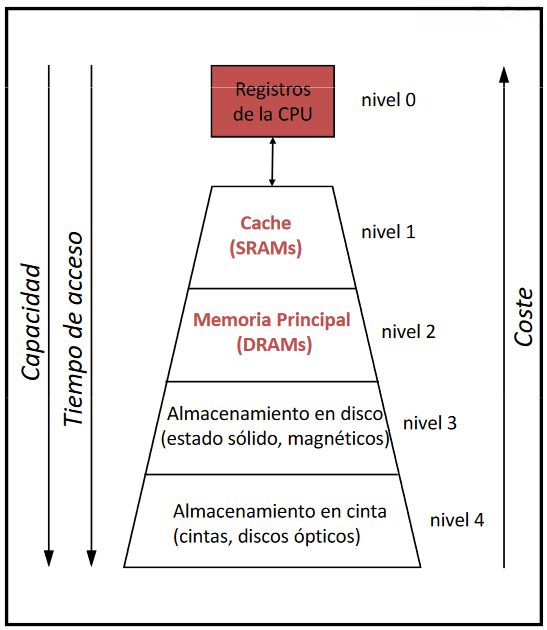
\includegraphics[width=0.4\textwidth]{images/Tema_5/Jerarquia_Memoria.PNG}
		\caption{Jerarquía de memoria}
	\end{figure}
\end{multicols}


Desde los años 90 el procesador trabaja más rápido que la memoria, tres de cada 4 ciclos se dedican a esperar a la memoria. Se necesitarán  más de 32 bytes cada 2 ns.

\begin{table}[H]
	\centering
	\begin{tabular}{|c|c|c|c|}
		\hline
		\textbf{Tipo de memoria} & \textbf{Bytes por acceso} & \textbf{Tiempo de acceso (ns)} & \$ por MByte \\
		\hline
		SRAM - Cache (on-chip)   & 10                        & 0.1                            & 1-100        \\
		\hline
		SRAM - Cache (off-chip)  & 100                       & 2-5                            & 1-10         \\
		\hline
		DRAM                     & 1000                      & 10-100                         & 0.1          \\
		\hline
		Disco magnético          & 1000                      & 5000000 - 2000000              & 0.001        \\
		\hline
	\end{tabular}
\end{table}

La diferencia de rendimiento entre procesadores y memorias ha ido incrementando en las últimas décadas.
\begin{figure}[H]
	\centering
	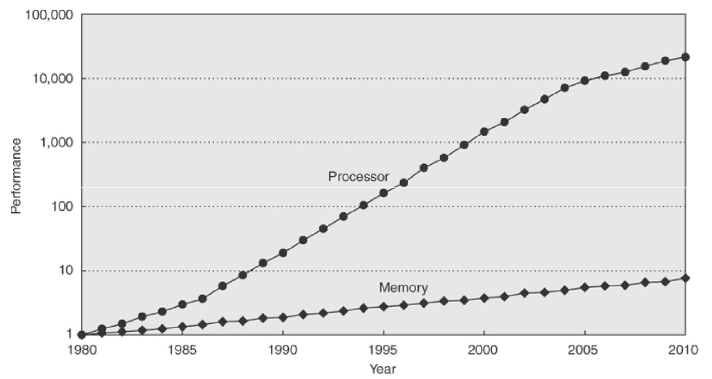
\includegraphics[width=0.5\textwidth]{images/Tema_5/Grafico_Memorias.PNG}
	\caption{Comparación de rendimiento entre procesadores y memorias a lo largo de los años}
\end{figure}


\section{Clasificación}
\subsection{Ubicación}
Se distinguen entre las memorias presentes en la \gls{cpu}(registros), las memorias internas (memoria cache) y memorias externas (memoria principal).
\subsection{Métodos de acceso}
Los principales métodos de acceso a la memoria son:

\begin{itemize}
	\item\textbf{Acceso directo:} la información está organizada en discos físicos apilados. Cada uno de ellos está dividido en pistas y cada una de ellas tiene varios cilindros. Un  grupo de cilindros concéntricos constituye un sector. El tiempo de acceso es variable, depende de la posición inicial de los cabezales del disco, respecto a la información que se va a leer.
	\item\textbf{Acceso aleatorio:} cada posición de memoria tiene un único método de acceso, que está cableado físicamente. El tiempo de acceso a memoria para una determinada posición de memoria es independiente de su dirección y de la secuencia de accesos previos a memoria.
	\item\textbf{Acceso asociativo:} las memorias asociativas son memorias de acceso aleatorio cuyas palabras no se acceden a través de ninguna dirección. Cada palabra lleva asociada un tag único(típicamente, el tag está asociado de alguna manera con la dirección, o al menos con parte de ella, donde esa palabra se almacena en otra memoria). Una palabra se puede guardar en cualquier lugar de la memoria, en otras palabras, la dirección específica donde se encuentra una palabra en un momento dado no es conocido. Por tanto, para acceder a una determinada información es necesario comprobar el tag de cada palabra en la memoria con el tag de la palabra que se desea buscar.
\end{itemize}

\subsection{Tecnologías de estado sólido}
\begin{itemize}
	\item \gls{sram}
	\item \gls{dram}
	\item \gls{sdram}
	\item \gls{eeprom}
	\item NAND-flash y NOR-flash
\end{itemize}


\section{Parámetros}

Los parámetros de medición en las memorias son:
\begin{itemize}
	\item\textbf{Tiempo de acceso (Ti):}
	      \begin{itemize}
		      \item En memorias de acceso aleatorio es el tiempo que transcurre desde que se especifica una dirección de memoria hasta que el dato ha sido almacenado o bien está disponible para su uso.
		      \item En memorias de acceso secuencial/directo es el tiempo que tarda en situar el mecanismo de lectura/escritura sobre la posición deseada.
	      \end{itemize}
	\item\textbf{Tiempo de ciclo de memoria:} es aplicable solo a memorias de acceso aleatorio. Es el tiempo mínimo que debe dejarse transcurrir entre dos accesos consecutivos. Es algo mayor que el tiempo de acceso.
	\item\textbf{Ancho de banda o velocidad de transferencia (Bi):} Velocidad a la que se puede transmitir datos desde/hacia una unidad de memoria. En memorias de acceso directo es igual a la inversa del tiempo de ciclo de memoria. En memorias de acceso secuencial/directo depende del tiempo de acceso medio y de la velocidad de transferencia del dispositivo.
	\item\textbf{Tamaño de la memoria (Si):} número de bytes que pueden almacenarse en el dispositivo de memoria.
	\item\textbf{Coste por byte (Ci):} coste medio estimado por cada byte de memoria. El coste total de un dispositivo de memoria viene dado por $Ci\times Si$.
	\item\textbf{Unidad de transferencia (Xi):} Unidad de información con las que trabaja un determinado dispositivo de memoria. Puede oscilar entre un byte o una palabra, hasta bloques de varios KBytes.
\end{itemize}

\begin{table}[H]
	\centering
	\begin{tabularx}{0.9\textwidth}{|p{3.5cm}|X|X|p{3cm}|X|}
		\hline
		\textbf{Nivel de jerarquía}    & \textbf{Acceso} & \textbf{Latencia} & \textbf{Coste(\$/MB)} & \textbf{Energía}  \\
		\hline
		On-chip cache                  & 10 B            & 100 ps            & 1-100                 & 1 nJ              \\
		\hline
		Off-chip cache                 & 100 B           & 1 ns              & 1-10                  & 10-100 nJ         \\
		\hline
		Memoria Principal (\gls{dram}) & 1000 B          & 10-100 ns         & 0.1                   & 1-100 nJ por chip \\
		\hline
		Disco duro                     & 1000 B          & 1 ms              & 0.001                 & 100-1000 mJ       \\
		\hline
	\end{tabularx}
	\caption{Comparativa entre distintos tipos de memorias}
\end{table}
\section{Tecnologías de memoria}
\subsection{\gls{sram}}
Esta es una \gls{ram} estática. Almacena un bit en un biestable, el valor permanece mientras la memoria tenga alimentación. La ventaja de la \gls{sram} es su rapidez, su inconveniente es que necesita 6 transistores, lo cual no permite alcanzar grandes densidades de integración.
\begin{multicols}{2}
	\begin{figure}[H]
		\centering
		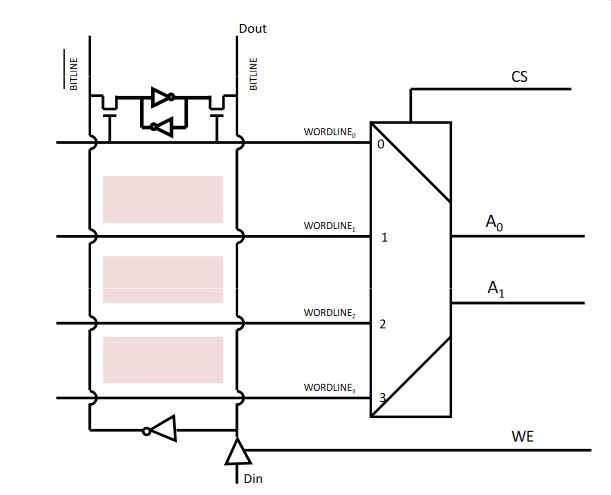
\includegraphics[width=0.4\textwidth]{images/Tema_5/Celda_Basica_Ram.PNG}
		\caption{Celda básica de la \gls{sram}}
	\end{figure}
	\vfill
	\null
	\begin{figure}[H]
		\centering
		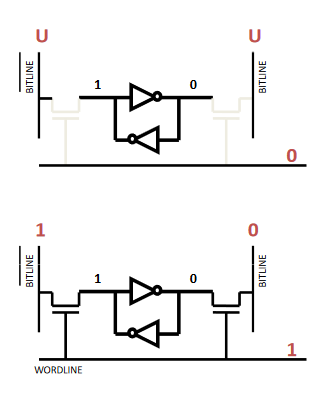
\includegraphics[width=0.4\textwidth]{images/Tema_5/Operacion_SRAM.PNG}
		\caption{Operación de la \gls{sram}}
	\end{figure}
	Cargamos o somos capaces de leer el valor almacenado si y sólo si WORDLINE vale 1.
\end{multicols}

\subsection{\gls{dram}}
Esta es una \gls{ram} dinámica. Almacena un bit en un condensador (cargado o descargado). El condensador pierde voltaje a lo largo del tiempo por lo que tiene que ser refrescado periódicamente, por eso se dice que es una memoria dinámica. La ventaja de las memorias \gls{dram} es su simplicidad, sólo se necesita un condensador y un transistor para almacenar un bit. Esto permite grandes densidades de integración. Es una memoria volátil, pierde rápidamente la información cuando se apaga.
\begin{multicols}{2}
	\begin{figure}[H]
		\centering
		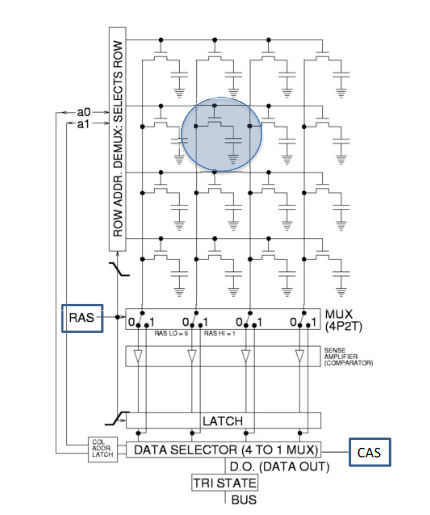
\includegraphics[width=0.4\textwidth]{images/Tema_5/Celda_Basica_Dram.PNG}
		\caption{Celda básica de una \gls{dram}}
	\end{figure}
	\textcolor{red}{LECTURA DESTRUCTIVA}\\
	Operación de lectura RAS: 0 leyendo / 1 escribiendo(leer dato)
	\vfill
	\null
	\begin{figure}[H]
		\centering
		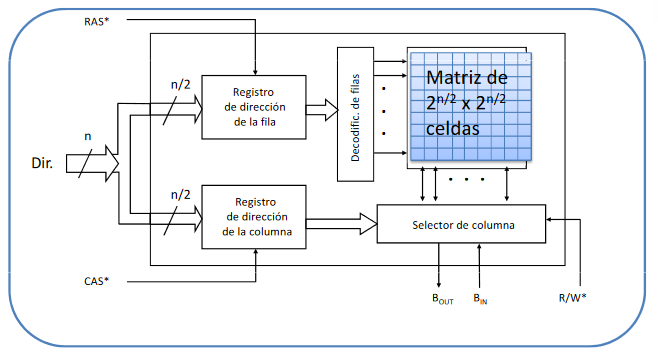
\includegraphics[width=0.4\textwidth]{images/Tema_5/Organizacion_Dram.PNG}
		\caption{Organización de una \gls{dram}}
	\end{figure}
	\textbf{RAS:} línea de selección de la fila

	\textbf{CAS:} línea de selección de la columna
\end{multicols}

\subsubsection{Lectura}
Las word-line se precargan con un nivel de voltaje entre 0  y 1 (se comportan como condensadores grandes) utilizando la mitad de la dirección que hace referencia a la fila. Este valor es mayor que el que está almacenado en las celdas \gls{dram}\\
Al recibir la señal RAS, se selecciona una fila y se establece una conexión entre una línea y los condensadores de las celdas. Las cargas iniciales de ambos condensadores son compartidas. La distribución de carga resultante sigue las siguientes reglas.
\[
	q_{1} + q_{2} = q'_{1} + q'_{2}
\]
\[
	\frac{q'_{1}}{c_{1}} = \frac{q'_{2}}{c_{2}}
\]
\noindent$q'_{1}$ y $q'_{2}$ serán diferentes dependiendo de la carga inicial de las celdas $q_{1}$ y $q_{2}$.
